\documentclass[journal,12pt,twocolumn]{IEEEtran}

\usepackage{setspace}
\usepackage{gensymb}

\singlespacing


\usepackage[cmex10]{amsmath}

\usepackage{amsthm}

\usepackage{mathrsfs}
\usepackage{txfonts}
\usepackage{stfloats}
\usepackage{bm}
\usepackage{cite}
\usepackage{cases}
\usepackage{subfig}

\usepackage{longtable}
\usepackage{multirow}

\usepackage{enumitem}
\usepackage{mathtools}
\usepackage{steinmetz}
\usepackage{tikz}
\usepackage{circuitikz}
\usepackage{verbatim}
\usepackage{tfrupee}
\usepackage[breaklinks=true]{hyperref}
\usepackage{graphicx}
\usepackage{tkz-euclide}
\usepackage{float}

\usetikzlibrary{calc,math}
\usepackage{listings}
    \usepackage{color}                                            %%
    \usepackage{array}                                            %%
    \usepackage{longtable}                                        %%
    \usepackage{calc}                                             %%
    \usepackage{multirow}                                         %%
    \usepackage{hhline}                                           %%
    \usepackage{ifthen}                                           %%
    \usepackage{lscape}     
\usepackage{multicol}
\usepackage{chngcntr}

\DeclareMathOperator*{\Res}{Res}

\renewcommand\thesection{\arabic{section}}
\renewcommand\thesubsection{\thesection.\arabic{subsection}}
\renewcommand\thesubsubsection{\thesubsection.\arabic{subsubsection}}

\renewcommand\thesectiondis{\arabic{section}}
\renewcommand\thesubsectiondis{\thesectiondis.\arabic{subsection}}
\renewcommand\thesubsubsectiondis{\thesubsectiondis.\arabic{subsubsection}}


\hyphenation{op-tical net-works semi-conduc-tor}
\def\inputGnumericTable{}                                 %%

\lstset{
%language=C,
frame=single, 
breaklines=true,
columns=fullflexible
}
\makeatletter
\setlength{\@fptop}{0pt}
\makeatother
\begin{document}
\newtheorem{theorem}{Theorem}[section]
\newtheorem{problem}{Problem}
\newtheorem{proposition}{Proposition}[section]
\newtheorem{lemma}{Lemma}[section]
\newtheorem{corollary}[theorem]{Corollary}
\newtheorem{example}{Example}[section]
\newtheorem{definition}[problem]{Definition}

\newcommand{\BEQA}{\begin{eqnarray}}
\newcommand{\EEQA}{\end{eqnarray}}
\newcommand{\define}{\stackrel{\triangle}{=}}
\bibliographystyle{IEEEtran}
\providecommand{\mbf}{\mathbf}
\providecommand{\ztrans}{\overset{\mathcal{Z}}{ \rightleftharpoons}}
\providecommand{\pr}[1]{\ensuremath{\Pr\left(#1\right)}}
\providecommand{\qfunc}[1]{\ensuremath{Q\left(#1\right)}}
\providecommand{\sbrak}[1]{\ensuremath{{}\left[#1\right]}}
\providecommand{\lsbrak}[1]{\ensuremath{{}\left[#1\right.}}
\providecommand{\rsbrak}[1]{\ensuremath{{}\left.#1\right]}}
\providecommand{\brak}[1]{\ensuremath{\left(#1\right)}}
\providecommand{\lbrak}[1]{\ensuremath{\left(#1\right.}}
\providecommand{\rbrak}[1]{\ensuremath{\left.#1\right)}}
\providecommand{\cbrak}[1]{\ensuremath{\left\{#1\right\}}}
\providecommand{\lcbrak}[1]{\ensuremath{\left\{#1\right.}}
\providecommand{\rcbrak}[1]{\ensuremath{\left.#1\right\}}}
\theoremstyle{remark}
\newtheorem{rem}{Remark}
\newcommand{\sgn}{\mathop{\mathrm{sgn}}}
\providecommand{\abs}[1]{\vert#1\vert}
\providecommand{\res}[1]{\Res\displaylimits_{#1}} 
\providecommand{\norm}[1]{\lVert#1\rVert}
%\providecommand{\norm}[1]{\lVert#1\rVert}
\providecommand{\mtx}[1]{\mathbf{#1}}
\providecommand{\mean}[1]{E[ #1 ]}
\providecommand{\fourier}{\overset{\mathcal{F}}{ \rightleftharpoons}}
%\providecommand{\hilbert}{\overset{\mathcal{H}}{ \rightleftharpoons}}
\providecommand{\system}{\overset{\mathcal{H}}{ \longleftrightarrow}}
	%\newcommand{\solution}[2]{\textbf{Solution:}{#1}}
\newcommand{\solution}{\noindent \textbf{Solution: }}
\newcommand{\cosec}{\,\text{cosec}\,}
\providecommand{\dec}[2]{\ensuremath{\overset{#1}{\underset{#2}{\gtrless}}}}
\newcommand{\myvec}[1]{\ensuremath{\begin{pmatrix}#1\end{pmatrix}}}
\newcommand{\mydet}[1]{\ensuremath{\begin{vmatrix}#1\end{vmatrix}}}
\numberwithin{equation}{subsection}
\makeatletter
\@addtoreset{figure}{problem}
\makeatother
\let\StandardTheFigure\thefigure
\let\vec\mathbf
\renewcommand{\thefigure}{\theproblem}
\def\putbox#1#2#3{\makebox[0in][l]{\makebox[#1][l]{}\raisebox{\baselineskip}[0in][0in]{\raisebox{#2}[0in][0in]{#3}}}}
     \def\rightbox#1{\makebox[0in][r]{#1}}
     \def\centbox#1{\makebox[0in]{#1}}
     \def\topbox#1{\raisebox{-\baselineskip}[0in][0in]{#1}}
     \def\midbox#1{\raisebox{-0.5\baselineskip}[0in][0in]{#1}}
\vspace{3cm}
\title{QUIZ 2}
\author{Vojeswitha Gopireddy \\ AI20BTECH11024}
\maketitle
\newpage
\bigskip
\renewcommand{\thefigure}{\theenumi}
\renewcommand{\thetable}{\theenumi}
Download all python codes from 
\begin{lstlisting}
https://github.com/V-Gopireddy/EE3900/blob/main/Quiz2/codes/Quiz-2.py
\end{lstlisting}
%
and latex-tikz codes from 
%
\begin{lstlisting}
https://github.com/V-gopireddy/EE3900/blob/main/Quiz2/Quiz-2.tex
\end{lstlisting}
\section{QUESTION 3.3(c)}
Determine the $z$-transform of the following sequence. Include with your answer the region of convergence in the $z$-plane and a sketch of the pole-zero plot. Express all sums in closed form.
\begin{align}
  x[n] = \begin{cases}
         n, & 0 \leq n \leq N \\~\\[-1em]
	     2N-n, & N+1 \leq n \leq 2N \\~\\[-1em]
	     0, & \text{otherwise}
         \end{cases}
\end{align}
%
\section{SOLUTION}
%
\begin{definition}\label{def:z}
    The $z$ tansform of a function is defined as
    \begin{align}
        x[n] & \ztrans X(z)\\
        X(z) &=\sum_{n=-\infty}^{\infty} x[n]z^{-n}
    \end{align}
\end{definition}

\begin{theorem}[Convolution Theorem] \label{ct}
Let $F(z)$ and $G(z)$ be the Z-transform of two functions $f$ and $g$ respectively. Then
\begin{align}
\mathcal{Z}(f * g)=F(z)G(z)
\end{align}
\end{theorem}
Given sequence is
\begin{align}
   x[n] = \begin{cases}
         n, & 0 \leq n \leq N \\~\\[-1em]
	     2N-n, & N+1 \leq n \leq 2N \\~\\[-1em]
	     0, & \text{otherwise}
         \end{cases}
\end{align}
%
Let's define a new sequence 
\begin{align}
    x_1[n] = \begin{cases}
         n, & 0 \leq n \leq N-1 \\~\\[-1em]
	     0, & \text{otherwise}
         \end{cases}
\end{align}
Consider
\begin{align}
    x_1[n]*x_1[n-1]
    &= \sum_{k = -\infty}^{\infty} x_1[k]x_1[n-1-k]
\end{align}
On solving we get,
\begin{align}
    x_1[n]*x_1[n-1] &= \begin{cases}
         n, & 0 \leq n \leq N \\~\\[-1em]
	     2N-n, & N+1 \leq n \leq 2N \\~\\[-1em]
	     0, & \text{otherwise}
         \end{cases}\\
    \implies x[n] &= x_1[n]*x_1[n-1] \label{lemma1} 
\end{align}
And,
\begin{align}
    X_1(z) &= \mathcal{Z}\{x_1(n)\} 
    = \sum_{n=0}^\infty z^{-n}\\
    &= \frac{1-z^{-N}}{1-z^{-1}}, z \neq 0
\end{align}
Therefore 
\begin{align}
        X_1(z) = \frac{1-z^{-N}}{1-z^{-1}}, ROC: z \neq 0
\end{align}
From \eqref{lemma1} we have,
\begin{align}
    x[n] &= x_1[n]*x_1[n-1]\\
     \implies X(z) &= \mathcal{Z}\{x_1[n]*x_1[n-1]\}\\
     &= X_1(z)\brak{z^{-1}X_1(z)}\\
     &= z^{-1}\brak{X_1(z)}^2\\
     &= z^{-1}\frac{(1-z^{-N})^2}{(1-z^{-1})^2}, z \neq 0
\end{align}
Therefore,
\begin{align}
    X(z) =  \mathcal{Z}\{x(n)\} = z^{-1}\frac{(1-z^{-N})^2}{(1-z^{-1})^2}
\end{align}
ROC in $z$-plane : $z \neq 0 $\\
Poles are,
\begin{align}
    z = 0 
\end{align}
Zeros exsist if N is even and they are:,
\begin{align}
    z = -1
\end{align}
\begin{figure}[h!]
\centering
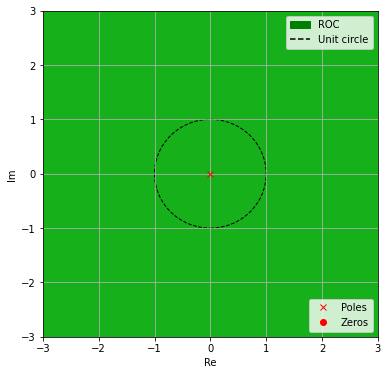
\includegraphics[width=\columnwidth]{pole-zeroPlot.png}
\caption{Pole-zero Plot of the given sequence}
\label{fig:ellipse}
\end{figure}
\end{document}